
\chapter{Separating Discriminative and Non-Discriminative Information for Semi-Supervised Learning}
\label{chapter:hybridnet}

\renewcommand{\leftmark}{\spacedlowsmallcaps{Separating Discriminative and Non-Discriminative Information}}

\begin{chapabstract}
	\acresetall
	{\em
  
  Regularizing \acfp{DNN} by encouraging invariance or by encouraging reconstruction are two popular methods with conflicting behaviors toward classification. In this chapter, we study those methods in more details and propose a new framework to make them cooperate in the context of \acf{SSL}, leveraging unlabeled data to improve generalization performances of image classifiers. To do so, we investigate ways to organize the information in the latent space and introduce a two-branch encoder-decoder architecture called HybridNet. The first branch of HybridNet receives supervision signal and is dedicated to the extraction of invariant class-related representations. The second branch is fully unsupervised and dedicated to model information  discarded by the first branch to reconstruct input data. To further support the expected behavior of our model, we propose an original training objective. It favors stability in the discriminative branch and complementarity between the learned representations in the two branches. At the time of publication, HybridNet was able to outperform state-of-the-art results on CIFAR-10, SVHN, and STL-10 in various semi-supervised settings. %In addition, visualizations and ablation studies validate our contributions and the behavior of the model on both CIFAR-10 and STL-10 datasets.

	\vspace*{5mm}
	The work in this chapter has led to the publication of a conference paper:}
	\begin{itemize}
		\item \small \fullcite{Robert2018}.
	\end{itemize}
\end{chapabstract}

\ifthenelse{\boolean{skipHN}}{\endinput}{}


\newpage

\minitoc
\chapterwithfigures{\nameref*{chapter:hybridnet}}
\chapterwithtables{\nameref*{chapter:hybridnet}}


\acused{SHADE}

\section{Introduction}


We have seen that \acp{DNN} and \acp{ConvNet} now show impressive state-of-the-art results on many \ac{CV} tasks (image classification \citep{he2016deep}, object localization \citep{dai2016r}, multimodal embedding \citep{Martin2018,Carvalho2018}, \etc). To achieve these results, important progress has been made to provide ways to regularize the huge number of parameters of \acp{DNN} (\eg weight decay, dropout, \ac{BN}, \etc.). In the previous chapter, we saw that these techniques mostly consist in introducing prior knowledge of models that should perform well; thus influencing the model's architecture, the smoothness of its decision boundary, its invariance capability, \etc. In this regard, we introduced \ac{SHADE} which proposes to encourage intra-class invariance. However, we also saw that another very interesting direction to regularize and improve \acp{ConvNet} is through \acf{SSL}.

Indeed, supervised learning of \acp{DNN} requires very large labeled datasets like ImageNet and its now 1.3 million images. Annotating such large quantities of data is very expensive and remains an obstacle to the application of those models to new tasks. Thus, in this chapter, we propose to tackle the problem of training \acp{DNN} using \acf{SSL}. In this context, only a small portion of our large dataset has labels, making it much less expensive since the cost of the dataset usually come from the expensive human annotation of the ground truth. This problem is particularly true in domains where the annotation process requires rare expertise such as the annotation of medical imagery. In such domains, annotated data is very rare and effective \ac{SSL} methods could be crucial. Indeed, the idea of \ac{SSL} is to take advantage of all the images (labeled or not) so that the model can grasp the diversity of the images it should be able to recognize, and simply use a few labeled images to effectively learn the classification rule, which will generalize better thanks to this more general knowledge of the dataset learned by the model.

As we saw in \autoref{shade:sec:RW_SSL}, the two main types of approaches for \ac{SSL} are as follows. The first one is by improving the quality of the model toward classification, introducing more invariance, often by enforcing stable predictions with regard to artificial sources of variability introduced by different stochastic perturbations \citep{Sajjadi2016,Laine2016,Tarvainen2017}. Compared to \ac{SHADE} which encourages intra-class invariance, those methods encourage intra-instance invariance to those stochastic perturbations. This criterion, not requiring any label, can be used on the unlabeled samples of the dataset to improve the quality of the features represented by the model.

\begin{figure}[t]
	\centering
	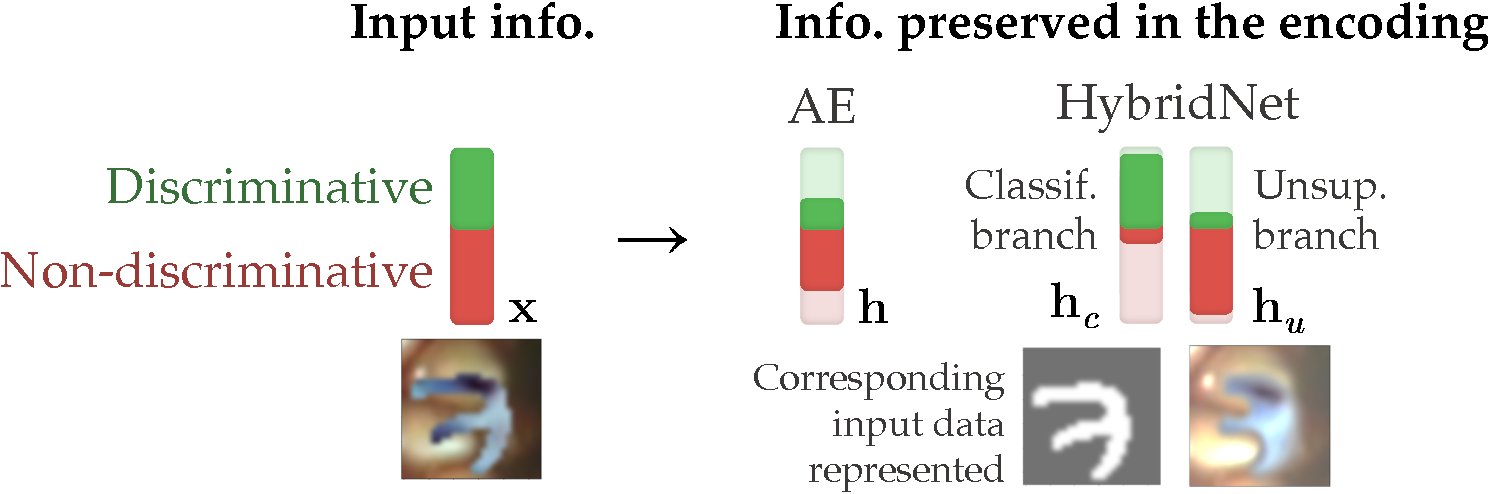
\includegraphics[width=0.8\textwidth]{images/hybridnet_intuition}
    \titlecaption{Illustration of how an \acs{AE} and HybridNet encode the information differently}{Considering an image contains discriminative and non-discriminative information represented on the left. On the right, we show the information preserved in the latent space of an \acs{AE} and of HybridNet. The auto-encoder will retain as much information as possible for reconstruction, possibly keeping lots of non-discriminative information necessary to optimize the \acs{MSE} loss. In HybridNet, we are able to preserve more information and organize it in the two branches, specializing $\vh_c$ on discriminative information and leaving $\vh_u$ to encode the non-discriminative one.}
    \label{hybridnet:fig:intuition}
\end{figure}


\begin{figure}[t]
	\centering
	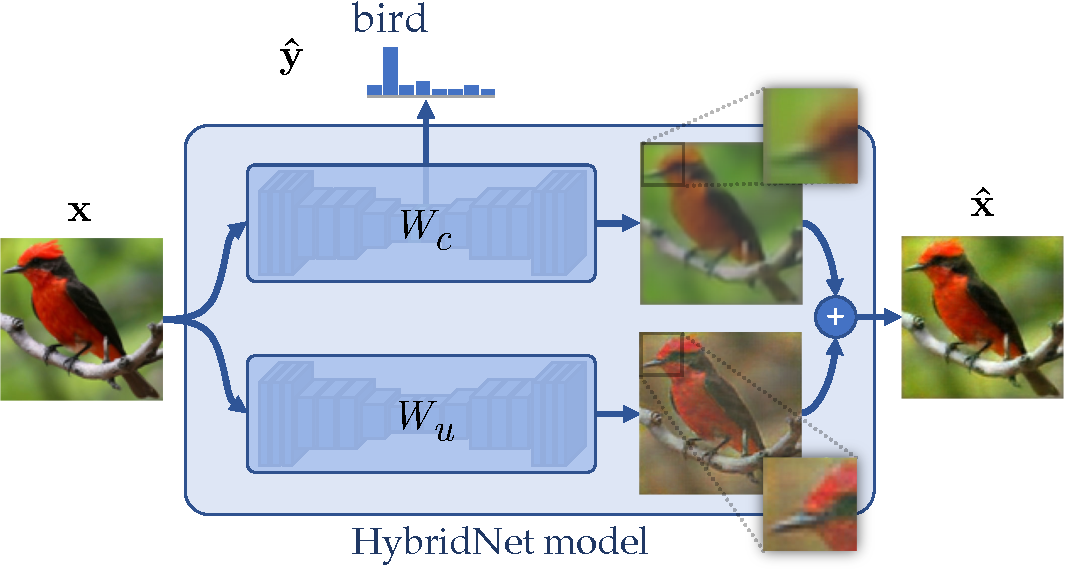
\includegraphics[width=0.7\textwidth]{images/hybridnet_overview}
    \titlecaption{Illustration of HybridNet's behavior}{The input image is processed by two network paths of weights $W_c$ and $W_u$; each path produces a partial reconstruction, and both are summed to produce the final reconstruction, while only one path is used to produce a classification prediction. Thanks to the joint training of both tasks, the weights $W_c$ and $W_u$ influence each other to cooperate.}
    \label{hybridnet:fig:intro}
\end{figure}


The second major direction is reconstruction- or generation-based methods \citep{bengio2007greedy}. In this case, the idea is that by making the model able to encode and decode all the images of the dataset, we obtain representations that model the whole distribution of images, even the ones for which we do not have a label. Thanks to this, we can produce more robust representations that will generalize better \citep{le2018supervised}. This strategy has been followed by historical deep learning approaches \citep{hinton2006reducing}, but also in some promising recent results with modern \acp{ConvNet} \citep{Zhang2016a}.

Those two directions seem to be complementarity since invariance improves classification and reconstruction should improve the generalization capabilities of the features. However, when we look more closely at the behavior of those techniques, they actually seem to have conflicting goals. Indeed, by definition, to reconstruct an image, all the information from the input is necessary. This information can be transformed, reshaped, but must be retained. On the other hand, classification and intra-class invariance regularizers tend to explicitly remove the information to achieve their goal.

In this chapter, we address this problem of conflict between classification and reconstruction, previously investigated by Ladder Networks \citep{Rasmus2015} for example. To solve it, we propose a new type of architecture and training that we call HybridNet. The general idea is illustrated in \autoref{hybridnet:fig:intuition}. Instead of having an auto-encoding model that will try to represent all the information in a single latent space $\vh$, we propose to split this information into two complementarity latent spaces $\vh_c$ and $\vh_u$. To do so, we design a ``hybrid'' \acf{AE} with a feature extraction path decomposed into two branches as represented in \autoref{hybridnet:fig:intro}. Thus, compared to a traditional \ac{AE}, the presence of the two branches allows separating discriminative and non-discriminative information. The first branch ($W_c$) producing $\vh_c$ is responsible for extracting discriminative information and to produce a class prediction, which is its main goal; it should thus extract invariant class-specific patterns as we have seen in \autoref{chapter:shade}. The second branch ($W_u$) is then here to capture the non-discriminative information that is not useful for classification. Combining both branches allows performing exact reconstruction without compromising the invariance properties of the discriminative branch.

In \autoref{hybridnet:sec:RW}, we present existing techniques to address \ac{SSL} that are the most related to HybridNet and present their limitations. We then present our HybridNet framework in \autoref{hybridnet:sec:model}. We then investigate its detailed behavior and capability to improve on state-of-the-art techniques (at time of publication) in \autoref{hybridnet:sec:experiements}.


\section{Reconstruction and Stability for Semi-Supervised Learning} \label{hybridnet:sec:RW}

We have seen in \autoref{shade:sec:RW_SSL} that \acf{SSL} is an interesting approach for regularizing \acfp{DNN} and improving the discriminative quality of their representations. We now propose to go over recent \ac{SSL} techniques that are most in relation to HybridNet.

As we described in \autoref{chapter:shade}, the usual framework of \ac{SSL} assumes that we have a partially labeled dataset $\mcD = \mcD_\mathrm{sup} \cup \mcD_\mathrm{unsup}$ with labeled pairs $\mcD_\mathrm{sup} = \{(\vx\kk, \vy\kk)\}_{k=1..N_\mathrm{s}}$ and unlabeled images $\mcD_\mathrm{unsup} = \{\vx\kk\}_{k=1..N_\mathrm{u}}$ and consider that the images of $\mcD_\mathrm{unsup}$ and $\mcD_\mathrm{sup}$ are drawn from the same distribution and all correspond to one of the known classes of $\mcD_\mathrm{sup}$. An \ac{SSL} training usually consists in mixing a supervised classification loss trained on $\mcD_\mathrm{sup}$ with an unsupervised regularization trained on the full dataset $\mcD$. Here, we focus on two main types of techniques: stability-based methods and reconstruction-based methods.

\subsection{Stability based methods}

A first unsupervised criterion for \ac{SSL} relies on increasing the stability and smoothness of the prediction function around the data points. As we have seen in \autoref{shade:sec:RW_regul}, this objective is fairly common to regularize \acp{DNN}, however, the goal here is to find a way to also take advantage of additional unlabeled images.

In particular, an original idea by \citet{Sajjadi2016} proposes to force the model to produce output prediction $\vyh$ that are stable toward many sources of variability to which the model should be invariant. The paper proposes to use heavy \ac{DA} (translation, rotation, shearing, noise, \textit{etc.}) and use a stochastic model containing dropout. The loss is designed so that all the outputs $\vyh^{(i,k)}$ should be the same for $k=1..K$, each $k$ representing a random variation of the same input $\vx^{(i)}$. This is measured by \ac{MSE} between all the pairs, for each image $i$:
\begin{equation}
  \mcL_\mathrm{stability} = \sum_{j=1}^K\sum_{k=1}^K||\vyh^{(i,k)} - \vyh^{(i,j)}||_2^2\,.
\end{equation}

This, however, has the drawback of requiring many passes of the same image to provide an effective regularization. To solve this, \citet{Laine2016,Tarvainen2017} both propose variants where the loss becomes, for an image $i$:
\begin{equation}
  \mcL_\mathrm{stability} = ||\vyh^{(i)} - \tilde{\vy}^{(i)}||_2^2\,,
\end{equation}
which can be seen as a special case of \citet{Sajjadi2016} where $K=2$ (called the $\Pi$ model) but now using a \textit{virtual} target $\tilde{\vy}^{(i)}$. \citet{Laine2016,Tarvainen2017} propose different solutions to obtain this virtual target, with the idea that this target will be more ``stable'' and thus more useful that the multiple targets of \citet{Sajjadi2016}.

\citet{Laine2016} propose Temporal Ensembling, defining $\tilde{\vy}^{(i)}$ as the exponential moving average of the previous outputs $\hat{\vy}^{(i)}$. If we consider the model constant, this would mean that the virtual target is an average of the outputs for the sample $i$ with many different random variants of $\vx^{(i)}$. Of course, because the model is changing by being trained, the behavior of this averaging is more complex because it also ``contains'' outputs produced by the model during past epochs.

To overcome this problem of averaging outputs over many epochs, \citet{Tarvainen2017} propose Mean Teacher, where instead of averaging outputs, the weights of the classification model $f_\vw$ are averaged over the previous batches to obtain the teacher model $f^\mathrm{MT}_\vw$. The virtual target is the output of this model: $\tilde{\vy}^{(i)} =  f^\mathrm{MT}_\vw(\vx^{(i)})$.
While the interpretation regarding stability becomes less clear, this relies on the property that averaged models are more stable and accurate. This model also retains the stability objective of the $\Pi$ model because $f_\vw$ and $f^\mathrm{MT}_\vw$ use independent random sources of variability.


\subsection{Reconstruction based methods}

The main limit of stability approaches is that their regularization effect only rely on the smoothing of the prediction function, encouraging the robustness and invariance of their features. However, they do not encourage the extraction of new and more general patterns using the appearance of the unlabeled images. This question is addressed by other approaches which explore the use of reconstruction in the \ac{SSL} context. By adding a decoder to the classifier and learning to reconstruct, it is possible to extract new and more robust features that more broadly model the full dataset, as we described in length in \autoref{shade:sec:RW_SSL_rec}.

Mixing a classification and a reconstruction cost has been used for a long time as a way to perform \ac{SSL} \citep[\eg\unskip][]{Ranzato2008}. This way, the classification decision can be learned on labeled samples $\mcD_\mathrm{sup}$ while features used to make the decision are learned on all the images in $\mcD$. Existing \ac{SSL} approaches can be based on \ac{AE} using reconstruction \citep{Weston2008,turian2010word} or on generative models that learn the data distribution, namely \ac{VAE} \citep{Kingma2014} and \acp{GAN} \citep{Springenberg2015,Denton2017,Bodla2018}.

However, as we mentioned, this strategy of mixing classification and reconstruction is questionable since they play contradictory roles. Classification arguably aims at extracting invariant class-specific features which induce an information loss detrimental for an effective reconstruction.
To overcome this issue, solutions have been proposed. A decade ago, \citet{Ranzato2007b} already proposed to address a specific component of this issue which is related to the localization of the visual information. Indeed, because encoders usually include max-pooling layers, this produces a loss of the spatial information that the decoder cannot guess. To overcome this issue, they provide the position of the max-poolings to the decoder to restore this information. This idea was applied more recently by \citet{Zhao2016a} in the model \acf{SWWAE}, designed for \ac{SSL} and based on an \ac{AE}.

Ladder Networks \citep{Rasmus2015} are another \ac{AE}-based attempt to overcome this, designing an encoder allowed to discard information thanks to noisy \textit{skip} connections to the decoder. Reconstruction at each layer of the decoder is produced using upper-layer representation and a noisy version of the reconstruction target. However, it is not obvious that providing a noisy version of the target and training the network to remove the noise allows the encoder to effectively remove information and produce invariant features, since it must be able to correct ``low-level'' errors that require specific information about the image instance being reconstructed.

The limit of those two approaches is that they explicitly provide \textit{by-passed} information to the decoder so that the encoder can discard this information, however, it is not clear if this is sufficient to allow the encoder to effectively produce intra-class invariant features. For example, while providing spatial information (in \ac{SWWAE}) is useful to enable translation invariance, the encoder still needs to represent lots of information that is not relevant for classification like detailed textures, shapes, \etc. For the Ladder Networks, as we have seen, it is not clear if providing a noisy version of the reconstruction target can allow the model to only encode intra-class invariant features. For example, the decoder must be able to correct a ``by-passed'' corrupted texture information by using ``normal'' information that must be represented by the encoder.

\subsubsection*{Notes on decoder design}

Finally, we can note that when using large modern \acp{ConvNet}, the problem of designing decoders able to invert an encoder still is an open question \citep{Wojna2017}. The usual solution is to mirror the architecture of the encoder by using \textit{transposed convolutions} \citep{dumoulin2016guide}, but this does not ensure that we will be able to reconstruct perfectly the original information.
This problem is exacerbated with irreversible pooling operations such as max-pooling that must be reversed by an upsampling operation. In \citet{Zhao2016a,Zhang2016a}, they use unpooling operations to bring back spatial information from the encoder to the decoder, reusing pooling switches locations for upsampling.
Another interesting option is to explicitly create models which are reversible by design. This is the option followed by recent works such as RevNet \citep{NIPS2017_6816} and i-RevNet \citep{jacobsen:hal-01712808}, being inspired by the second generation of bi-orthogonal multi-resolution analysis and wavelets \citep{swe:spie95} from the signal processing literature.

\section{HybridNet framework}
\label{hybridnet:sec:model}

In this section, we detail our contributions with the HybridNet framework, that are twofold: first, in \autoref{hybridnet:sec:archi}, we propose an architecture designed to efficiently make reconstruction and classification losses cooperate; second, in \autoref{hybridnet:sec:training}, we design a training loss adapted to it that includes reconstruction, stability in the discriminative branch and a branch complementarity technique. This framework will then be validated on CIFAR-10, SVHN and STL-10 datasets in \autoref{hybridnet:sec:experiements}.

\subsection{Designing the HybridNet architecture}
\label{hybridnet:sec:archi}

\subsubsection{Separating visual information in two latent spaces}

%\note{exposition du problème}
As we have seen, a model designed for both classification and reconstruction faces a conflict in the features it should encode. For classification, a model will tend to filter out non-discriminative information, removing possibly a large part of the visual data to produce intra-class invariance features. This is of course especially true when using regularization that adds invariance. On the other hand, reconstruction needs to preserve all the information in a compact representation, and then decompress this representation into the reconstruction. If the same latent space is used for both tasks, a clear competition between the two losses arise.

%\note{positionnement par rapport a LN/SWWAE}
Previous methods addressing this problem \citep{Rasmus2015,Zhao2016a,Zhang2016a} mostly propose to add direct skip connections from the encoder to the decode to provide pooling locations information or a noisy version of the reconstruction target. Unlike those approaches, with HybridNet, we choose to propose an explicit separation of the information in two distinct learned spaces, which should allow for a finer and learned separation of discriminative and non-discriminative features, and is thus expected to have a more favorable impact on producing discriminative features. HybridNet also differs from reversible models \citep{NIPS2017_6816,jacobsen:hal-01712808} by having an explicit separation between the two latent spaces, which is complicated to achieve in reversible models due to the their particular design. Another difference is that HybridNet is allowed to discard information. Reversible models, by design, cannot discard any information but can only deform the input manifold into a new one, as opposed to the usual idea of introducing invariance in the representations.

\begin{figure}[t]
  \begin{subfigure}[t]{0.47\linewidth}
    \centering
    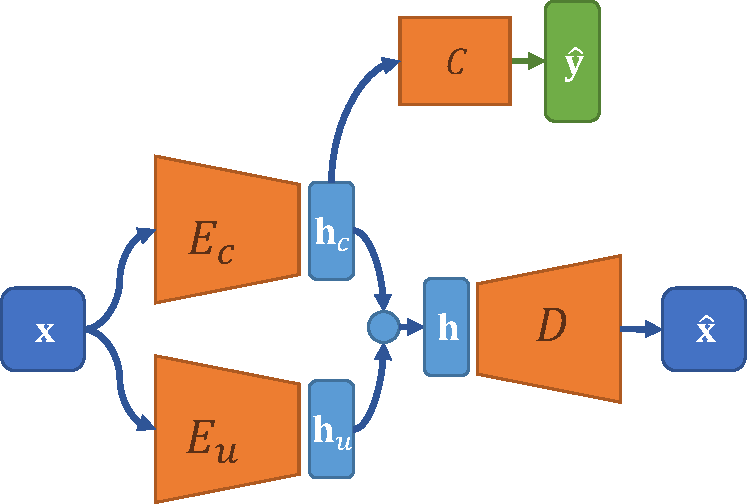
\includegraphics[height=4.5cm]{images/hybridnet_merge_early}
    \titlecaption[c]{Early fusion}{merging the representations and using a single decoder.}
    \label{hybridnet:fig:fusion_early}
  \end{subfigure}
  \hfill
  \begin{subfigure}[t]{0.47\linewidth}
    \centering
    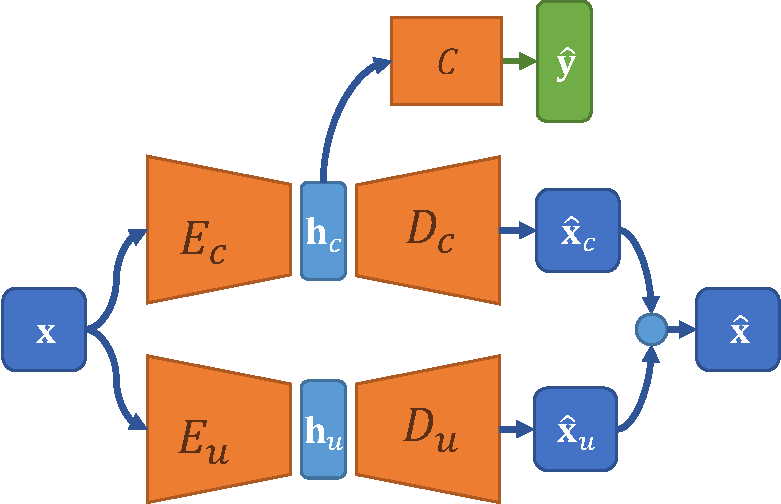
\includegraphics[height=4.5cm]{images/hybridnet_merge_late}
    \titlecaption[c]{Late fusion}{using two decoders and merging the reconstructions.}
    \label{hybridnet:fig:fusion_late}
  \end{subfigure}
  \titlecaption[c]{Overview of the architecture of HybridNet}{\unskip, with the two main possible fusion process for merging the two branches. The blue dot \begin{tikzpicture}\draw[lightblueborder,fill=lightbluefill,line width=1pt] circle(0.6ex);\end{tikzpicture} symbolizes the fusion operation, like concatenation or addition, but more complex fusion methods could be used.}
  \label{hybridnet:fig:fusion}
\end{figure}


%\note{idea vs AE}
As we illustrated in \autoref{hybridnet:fig:intuition} (page \pageref{hybridnet:fig:intuition}), the idea of HybridNet consists in using a ``hybrid'' \acf{AE} with the feature extraction path decomposed in two complementarity branches. Compared to a traditional \ac{AE}, the presence of the two-branches allows separating discriminative and non-discriminative information. 

%\note{role de la branch discr.}
Taking the example of the architecture in \autoref{hybridnet:fig:fusion_early}, the \textit{discriminative encoder} $E_c$ (top) produces $\vh_c$ and is connected to a classification block $C$ that produces class predictions $\vyh$, which is the main goal of this branch. This encoder should thus ideally focus on discriminative features that are expected to extract invariant class-specific patterns for a better generalization, as we have seen in \autoref{chapter:shade}. In this case, part of the information is lost in this branch and exact reconstruction from it should not be possible.

%\note{role de la branch unsup}
To complement this encoder and capture the missing information, a second \textit{unsupervised encoder} $E_u$ (bottom) is added and produces $\vh_u$. It is only by combining the information in $\vh_c$ and $\vh_u$ that we are able to produce a complete reconstruction $\vxh$.
%
During training, the supervised classification cost impacts the weights of $E_c$ while an unsupervised reconstruction cost is applied to both $E_c$ and $E_u$ to properly reconstruct the input image. The main assumption behind HybridNet is that this two-path architecture helps in making classification and reconstruction cooperate.

%\note{complémentarité}
An important goal of HybridNet is to produce encoders with complementary roles. The discriminative path must extract discriminative features $\vh_c$ that should eventually be well crafted to effectively perform a classification task, without being able to  produce a full reconstruction since preserving all the information is not a behavior we want to encourage. Consequently, the role of the unsupervised path is to be complementary to the discriminative branch by retaining in $\vh_u$ the information lost in $\vh_c$. The general HybridNet architecture can thus be described with the following equations:
\begin{align}\label{hybridnet:eq:general}
	\vh_c &= E_c(\vx) & \vyh &= C(\vh_c) & \vh_u &= E_u(\vx) & \vxh &= D(\vh_c, \vh_u)\,.
\end{align}

%\note{reconstruction as a regul}
It is important to note that the end-role of reconstruction here is just to act as a regularizer for the discriminative encoder $E_c$. However, as we have seen, complete reconstruction is a too strong regularization since it requires to retain too much information. Our unsupervised path via $E_u$ is the key element that gives freedom to the discriminative branch to take advantage of additional data while still being able to filter out information and to perform the target task of classification.

%\note{RW vs wavelet} 
Interestingly, this idea of separating the information in two subspaces and combining it for reconstruction also has conceptual connections to wavelet decomposition \citep{wavelets}: the first branch can be seen as extracting discriminative low-pass features from input images, and the second branch acting as a high-pass filter to restore the lost information.

\subsubsection{Merging the information for reconstruction}

After separating the information in two latent spaces, arise the question of how to merge back the information to produce the final reconstruction. Indeed, the decoding part of our model $D(\vh_c, \vh_u)$ (\cf \autoref{hybridnet:eq:general}) must produce the reconstruction by merging the information from the two latent spaces. To do so, we have two main possibilities: an early fusion (\cf \autoref{hybridnet:fig:fusion_early}), merging directly $\vh_c$ and $\vh_u$ and then producing the reconstruction; or a late fusion (\cf \autoref{hybridnet:fig:fusion_late}), where each representation is decoded independently by a specific decoder, giving partial reconstructions $\vxh_c$ and $\vxh_u$ that are then merged into $\vxh$.

%\note{Early fusion.}
With early fusion, the equations describing the architecture are:
\begin{equation}
  \vh = \mathrm{merge}(\vh_c, \vh_u)\,, \qquad \vxh = D(\vh)\,.
\end{equation}
Using an early fusion has the advantage of using a single decoder $D$ that has all the information available and can combine it freely to produce the reconstruction. Thus, this decoder can find complex combinations and interactions between the two latent spaces to solve its task. In addition, we can introduce prior knowledge in the choice of the $\mathrm{merge}$ function, which are numerous. The simplest solutions are a merge by addition, concatenation or element-wise product. Each of these solutions has its own semantic: addition enforces that representations have additive values in a shared latent space, concatenation would be an extension of addition where the first layer learns linear combinations of both representations, and multiplication can be interpreted as a weighting or attention mechanism between the two. More complex merging strategies could also be used, such as using bilinear combinations of $\vh_c$ and $\vh_u$ \citep{benyounescadene2017mutan,paumard2018jigsaw}. This merging method could model complex relations between the two spaces and would give the ability to the encoders to produce strongly semantic latent representations that could interact with each other. For example, semantic information about the class of the image (\eg a car) could be combined with semantic information regarding the style of the object (\eg the design and color) to effectively reconstruct a specific object on the input.

%\note{Late fusion.}
With late fusion, the equations are:
\begin{equation}
	\vxh_c = D_c(\vh_c)\,,\qquad \vxh_u = D_u(\vh_u)\,,\qquad \vxh = \mathrm{merge}(\vxh_c, \vxh_u)\,.
\end{equation}
In this case, a first advantage is that each decoder can be designed symmetrically to its corresponding encoder, as is common when designing \ac{AE}. In addition to simplifying the design of the architecture, it also provides additional control over the behavior of the model. For example, we can use the location of the max-pooling layers in the encoder to use in the corresponding upsampling layer of the decoder \citep{Zhao2016a}. We can also introduce intermediate reconstruction costs as we will see. Finally, we can ensure that both branches are contributing to the final reconstruction, which is much more complex to do with an early fusion. Using late fusion, we also have the question of how to merge the two partial reconstructions. The easiest solution is to merge them by addition in the pixel space, similarly to what is done with wavelet decomposition. But more complex merge techniques could be used to enforce specific semantics to partial reconstructions through a specific merge strategy, as is proposed by some methods \citep{shu2017neural,Shu_2018_ECCV,luvizon2017human}. For example, it could be interesting to investigate the use of a sort of soft attention or masking mechanism, with one branch creating the textures and the other creating the shape. Such an handcrafted mechanism should however be carefully designed to be aligned with the goal of $E_c$ and the production of discriminative features which is not obvious.

%\paragraph{Advantages and drawbacks.}
%\note{conclu}
In this situation, the drawbacks of one solution are the absence of the advantages proposed by the other. On one side, early fusion seems to enable more complex complementarity between the two spaces. On the other side, late fusion provides much more control over the behavior of the model.
%
%\note{cooperation challenge}
And actually, an important and interesting challenge of HybridNet is to find a way to ensure that the two branches will, in fact, behave in this desired way. The two main issues that we tackle are the fact that we want the discriminative branch to focus on discriminative features, and that we want both branches to cooperate and contribute to the reconstruction. Indeed, in both cases, we can end up with two paths that work independently: a classification path being $\vyh = C(E_c(\vx))$; and a reconstruction path being $\vxh = D(\vh_c)$ with $\vh_u$ not intervening in $D$ for early fusion or $\vxh = \vxh_u = D_u(E_u(\vx))$ and $\vxh_c = 0$ for late fusion.

Solving those two issues is achieved both through the choice of the architecture of HybridNet and the development of a well-designed training loss to control the behavior of HybridNet. While we tried both fusion strategies, late fusion is more adapted to solve this problem. For this reason, the rest of the architecture will be explained for this kind of fusion, using a merge by addition in the pixel space. On the other hand, early fusion will be further explored in \autoref{chapter:dualdis} in the context of disentangling.


\subsubsection{Designing a dual decoder HybridNet}

\begin{figure}[t]
  \centering
  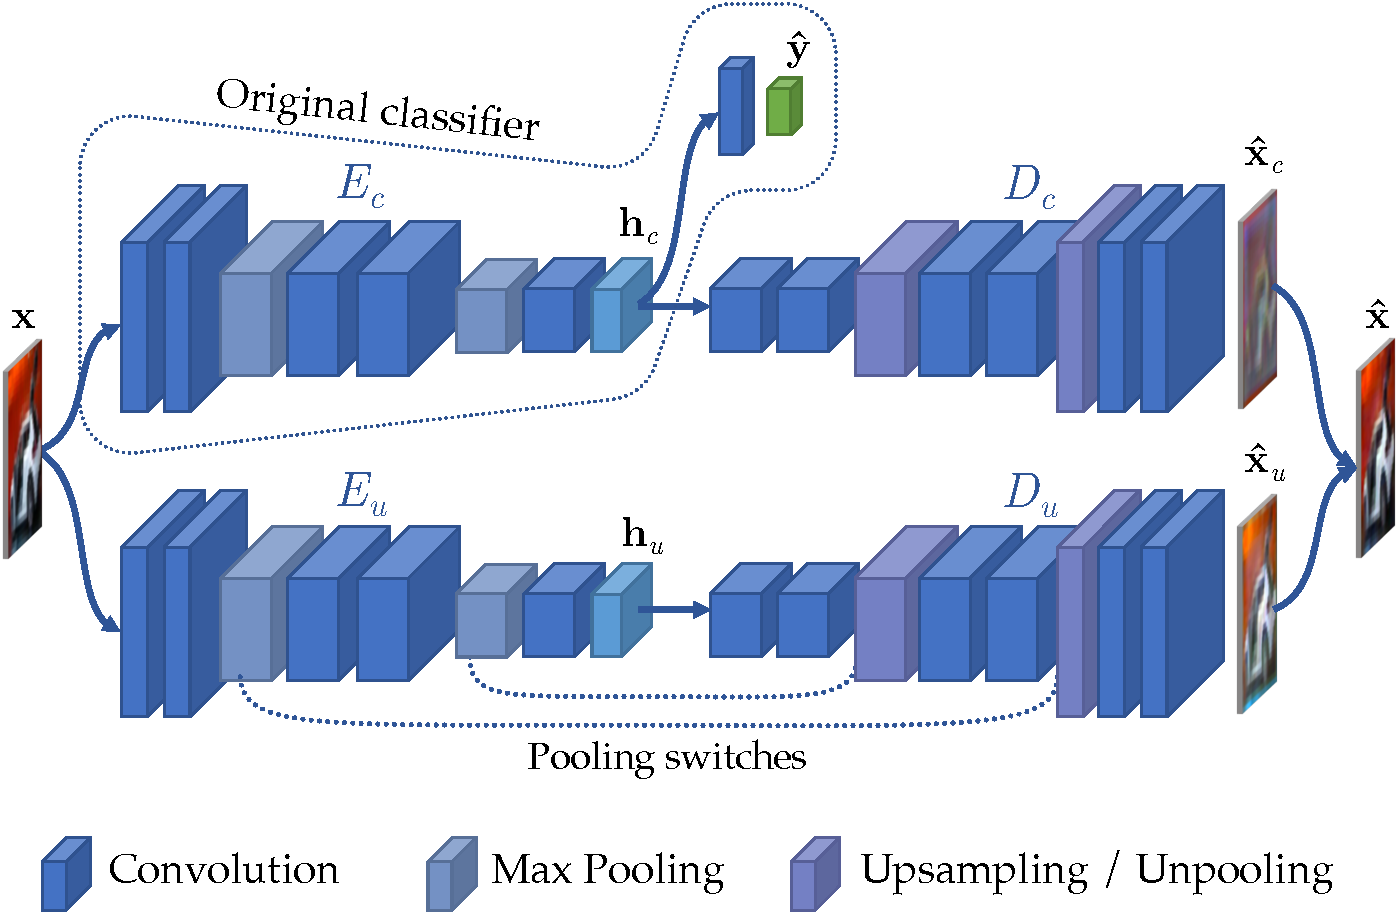
\includegraphics[width=0.85\textwidth]{images/hybridnet_archi_example}
  \titlecaption{Example of a detailed HybridNet architecture using late fusion}{We represent the output feature maps of convolutions, max-pooling and unpooling/upsampling layers.}
  \label{hybridnet:fig:archi_example}
\end{figure}


Let us now describe more thoroughly the architecture of a HybridNet using late fusion, \ie with two complete separate encoding-decoding paths, merging partial reconstructions by addition. An example of HybridNet architecture is presented in \autoref{hybridnet:fig:archi_example}, described with the following equations:
\begin{align}		
	\vh_c &= E_c(\vx) & \vxh_c &= D_c(\vh_c) & \vyh &= C(\vh_c)\\		
	\vh_u &= E_u(\vx) & \vxh_u &= D_u(\vh_u) & \vxh &= \vxh_c + \vxh_u		
\end{align}	

To design the HybridNet architecture, we start with a convolutional architecture adapted to the targeted dataset, for example a state-of-the-art ResNet architecture for CIFAR-10. This architecture is split into two modules: the discriminative encoder $E_c$ and the classifier $C$. On top of this model, we add the discriminative decoder $D_c$.
The location of the splitting point in the original network is free, but $C$ will not be directly affected by the reconstruction loss. In our experiments, we choose $\vh_c$ ($E_c$'s output) to be the last intermediate representation before the final pooling that aggregates all the spatial information, leaving in $C$ a global average pooling followed by one or more fully-connected layers.

The decoder $D_c$ is designed to be a ``mirror'' of the encoder's architecture, as commonly done in the literature, \textit{e.g.} \citep{Zhao2016a,Rasmus2015,zeiler2014visualizing}. This means that all the convolutional layers (with unit stride) are replaced by similar convolutions with swapped input/output planes number and in the reverse order. Pooling layers or strides convolutions, that reduce the spatial size, can be reversed using upsampling (or \textit{transposed} convolutions \citep[\textit{cf.}][]{dumoulin2016guide} that can be seen as a special upsampling followed by a regular convolution) or unpooling as we will see.

After constructing the discriminative branch, we add an unsupervised complementary branch. To ensure that both branches are ``balanced'' and behave in a similar way, the internal architecture of $E_u$ and $D_u$ is mostly the same as for $E_c$ and $D_c$.
The only difference remains in the mirroring of pooling layers, using either upsampling or unpooling. An upsampling will increase the spatial size of a feature map without any additional information while an unpooling, used by \citet{Zhao2016a,Zhang2016a}, will use spatial information (\textit{pooling switches}) from the corresponding max-pooling layer to do the upsampling. In our architecture, we propose to use upsampling in the discriminative branch because we want to encourage spatial invariance, and use unpooling in the unsupervised branch to compensate this information loss and favor the learning of spatial-dependent low-level information.

As mentioned previously, one key problem to tackle is to ensure that this model will behave as expected, \textit{i.e.} by learning discriminative features in the discriminative encoder and non-discriminative features in the unsupervised one.
This is encouraged by different ways in the design of the architecture. First, the fact that only $\vh_c$ is used for classification means that $E_c$ will be pushed by the classification loss to produce discriminative features. Thus, the unsupervised branch will naturally focus on information lost by $E_c$. Using upsampling in $D_c$ and unpooling in $D_u$ also encourages the unsupervised branch to focus on low-level information. In addition to this, the design of an adapted loss and training protocol is a major contribution to the efficient training of HybridNet.


\subsection{Training HybridNet}
\label{hybridnet:sec:training}

\begin{figure}[t]
	\centering
	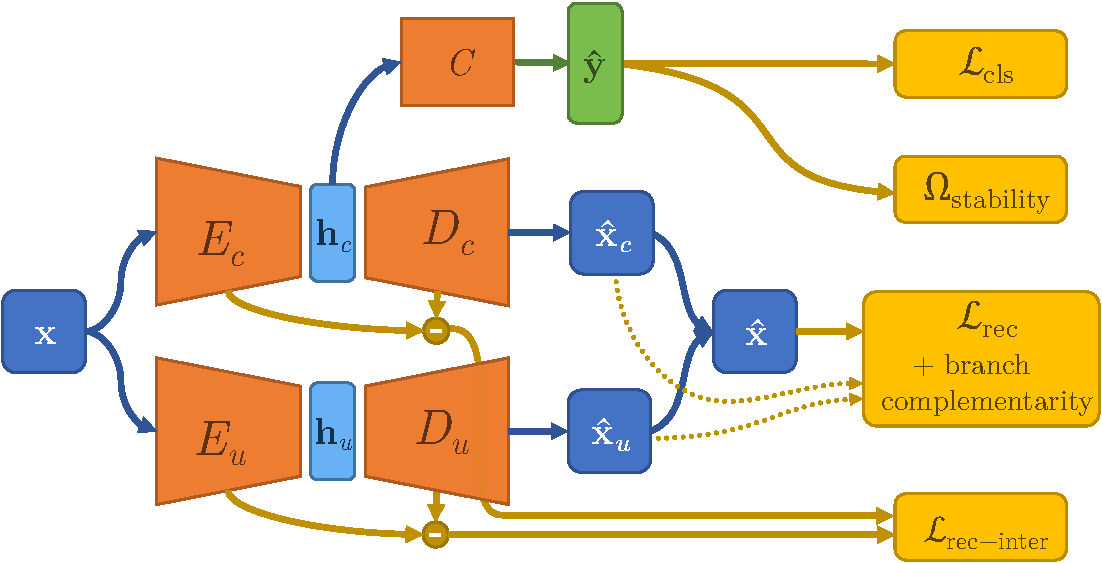
\includegraphics[width=0.8\textwidth]{images/hybridnet_losses}
  \titlecaption{General description of the HybridNet framework}{$E_c$ and $C$ correspond to a classifier, $E_c$ and $D_c$ form an autoencoder that we call \textit{discriminative path}, and $E_u$ and $D_u$ form a second autoencoder called \textit{unsupervised path}. The various loss functions used to train HybridNet are also represented in yellow.}
    \label{hybridnet:fig:general-archi}
\end{figure}


The HybridNet architecture has two information paths with only one producing a class prediction and both producing partial reconstructions that should be combined. In this section, we address the question of training this architecture efficiently. The complete loss is composed of various terms as illustrated in \autoref{hybridnet:fig:general-archi}. It comprises terms for classification with $\mathcal L_\mathrm{cls}$; final reconstruction with ${\mathcal L_\mathrm{rec}}$; intermediate reconstructions with ${\mathcal L_\mathrm{rec-inter}}_{b,l}$ (for layer $l$ and branch $b$); and stability with $\Omega_\mathrm{stability}$. It is also accompanied by a branch complementarity training method. Each term is weighted by a corresponding parameter $\lambda$:
\begin{equation}\textstyle
	\mathcal L = \lambda_\mathrm{c} \mathcal L_\mathrm{cls} + \lambda_\mathrm{r} \mathcal L_\mathrm{rec} + \sum_{b\in \{c,u\},l} {\lambda_\mathrm{r}}_{b,l} {\mathcal L_\mathrm{rec-inter}}_{b,l} + \lambda_\mathrm{s} \Omega_\mathrm{stability} \,.
    \label{hybridnet:eq:full-loss}
\end{equation}

HybridNet can be trained on a partially labeled dataset, \textit{i.e.} that is composed of labeled pairs $\mathcal D_\mathrm{sup} = \{(\vx\kk, \vy\kk)\}_{k=1..N_\mathrm{s}}$ and unlabeled images $\mathcal D_\mathrm{unsup} = \{\vx\kk\}_{k=1..N_\mathrm{u}}$.
Each batch is composed of $n$ samples, divided into $n_\mathrm{s}$ image-label pairs from $\mathcal D_\mathrm{sup}$ and $n_\mathrm{u}$ unlabeled images from $\mathcal D_\mathrm{unsup}$.

\subsubsection{Classification}

The classification term is a regular cross-entropy term, that is applied only on the $n_s$ labeled samples of the batch and averaged over them:
\begin{equation}
	\ell_\mathrm{cls}(\vyh, \vy) = \ell_\mathrm{CE}(\vyh, \vy) = -\sum_i \vy_i \log \vyh_i \, , \qquad \mathcal L_\mathrm{cls}=\frac{1}{n_s} \sum_k \ell_\mathrm{cls}(\vyh\kk, \vy\kk) \ .
\end{equation}

\subsubsection{Reconstruction losses}

We saw that in HybridNet, we mostly choose to keep discriminative and unsupervised paths separate so that they produce two complementary reconstructions $(\vxh_u, \vxh_c)$ that we combine with an addition into $\vxh = \vxh_u + \vxh_c$. Keeping the two paths independent until the reconstruction in pixel space, as well as the merge-by-addition strategy, allows us to apply different treatments to them and influence their behavior efficiently. The reconstruction loss that we use is a simple \ac{MSE} between the input and the sum of the partial reconstructions:
\begin{equation}
	\ell_\mathrm{rec} = ||\vxh - \vx||_2^2 = ||\vxh_u + \vxh_c - \vx||_2^2\,, \qquad \mathcal L_\mathrm{rec}=\frac{1}{n} \sum_k \ell_\mathrm{rec}(\vxh\kk, \vx\kk) \ .
\end{equation}

In addition to the final reconstruction loss, we also add reconstruction costs between intermediate representations in the encoders and the decoders which is possible since encoders and decoders have mirrored structure. We apply these costs to the representations $\vh_{b,l}$ (for branch $b$ and layer $l$) produced just after pooling layers in the encoders and reconstructions $\vhh_{b,l}$ produced just before the corresponding upsampling or unpooling layers in the decoders. This is common in the literature \citep{Zhao2016a,Zhang2016a,Rasmus2015} but is particularly important in our case: in addition to guiding the model to produce the right final reconstruction, it pushes the discriminative branch to produce a reconstruction and avoid the undesired situation where only the unsupervised branch would contribute to the final reconstruction. This is applied in both branches ($b \in \{c,u\}$):
\begin{equation}
	{\mathcal L_\mathrm{rec-inter}}_{b,l} = \frac{1}{n} \sum_k ||\vhh_{b,l}\kk - \vh_{b,l}\kk||_2^2\,.
\end{equation}


\subsubsection{Branch cooperation}

\begin{figure}[t]
	\centering
	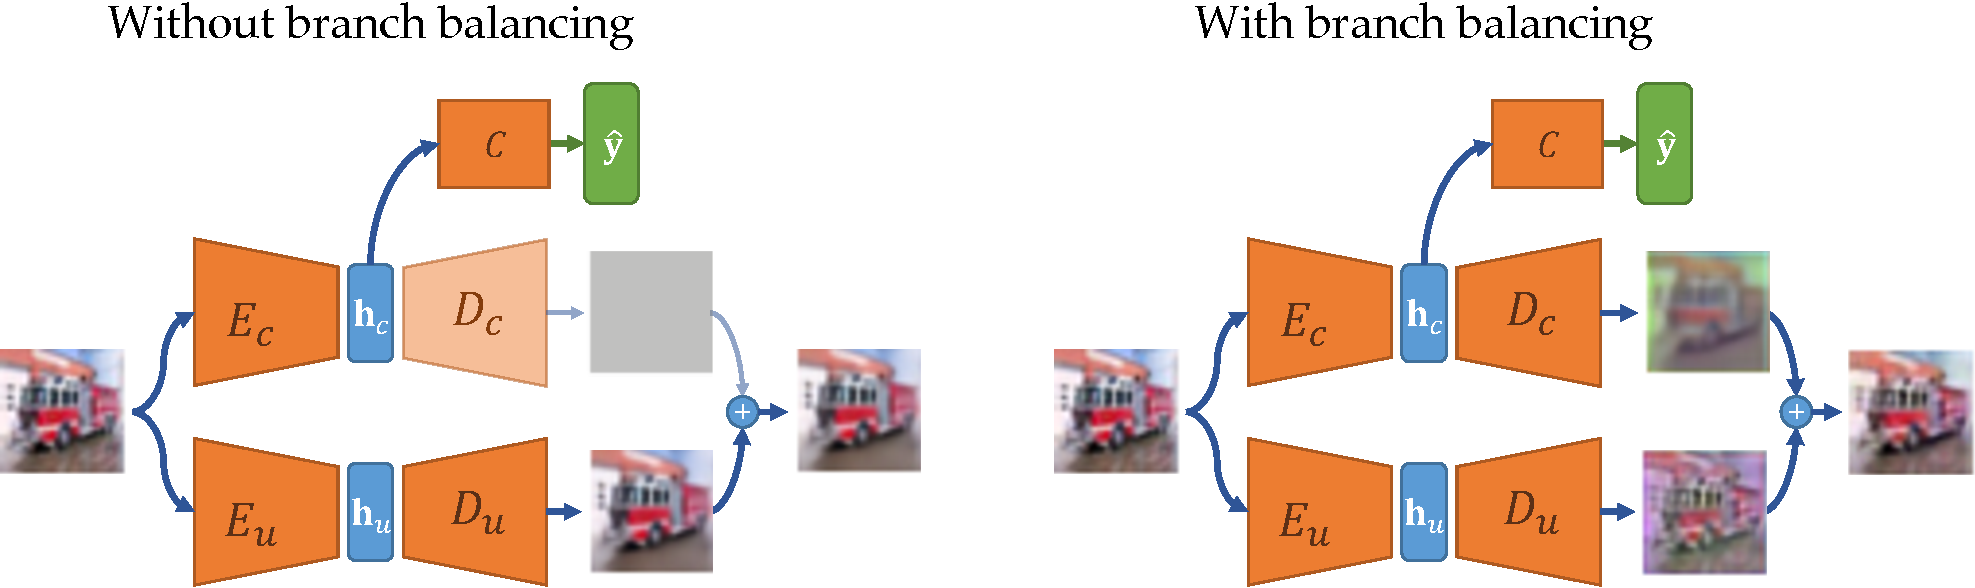
\includegraphics[width=\textwidth]{images/hybridnet_balacing}
  \titlecaption{Illustration of the effect of branch balancing on reconstructions}{Without branch balancing, the model can learn two separate paths, classifying with $E_c$ and reconstructing with $D_u\circ E_u$ without using $\vh_c$. The branch balancing forces both branches to produce a reconstruction and ensures that $E_c$ is regularized by the reconstruction loss.}
    \label{hybridnet:fig:balancing}
\end{figure}

As described previously, we want to ensure that both branches contribute to the final reconstruction, otherwise, this would mean that the reconstruction is not helping to regularize $E_c$, which is our end-goal. Having both branches produce a partial reconstruction and using intermediate reconstructions already help with this goal. In addition, to balance their training even more, we propose a training technique such that the reconstruction loss is only backpropagated to the branch that contributes less to the final reconstruction of each sample. This is done by comparing $||\vxh_c - \vx||_2^2$ and $||\vxh_u - \vx||_2^2$ and only applying the final reconstruction loss to the branch with the higher error. The expected effect of this branch balancing strategy is shown in \autoref{hybridnet:fig:balancing}.

This can be implemented either in the gradient descent or simply by preventing gradient propagation in one branch or the other using features like \texttt{tf.stop\_gradient} in Tensorflow or \texttt{.detach()} in PyTorch:
\begin{equation}
	\mathcal \ell_\mathrm{rec-balanced} = \begin{cases}
    	||\vxh_u + \mathrm{stopgrad}(\vxh_c) - \vx||_2^2&\text{if }||\vxh_u - \vx||_2^2 \geq ||\vxh_c - \vx||_2^2\\
        ||\mathrm{stopgrad}(\vxh_u) + \vxh_c - \vx||_2^2&\text{otherwise}\\
    \end{cases} .
\end{equation}

\subsubsection{Encouraging invariance in the discriminative branch}

We have seen that an important issue that needs to be addressed when training this model is to ensure that the discriminative branch will filter out information and learn invariant features. For now, the only signal that pushes the model to do so is the classification loss. However, in a semi-supervised context, when only a small portion of our dataset is labeled, this signal can be fairly weak and might not be sufficient to make the discriminative encoder focus on invariant features.

A first option to encourage invariance would be to use \ac{SHADE}. As presented in \autoref{chapter:shade}, \ac{SHADE} is designed to maximize the intra-class invariance of the features. As such, it is a good candidate for our purpose and could be applied to the discriminative encoder $E_c$.
 
The second option is to use a \textit{stability regularizer}. Such a regularizer is currently at the core of the models that give state-of-the-art results in a semi-supervised setting on the most common datasets \citep{Sajjadi2016,Laine2016,Tarvainen2017}. The principle is to encourage the classifier's output prediction $\vyh\kk$ for sample $k$ to be invariant to different sources of randomness applied on the input (translation, horizontal flip, random noise, \textit{etc.}) and in the network (\textit{e.g.} dropout). This is done by minimizing the \ac{MSE} between the output $\vyh\kk$ and a ``stability'' target $\tilde{\vy}\kk$. Multiple methods have been proposed to compute such a target \citep{Sajjadi2016,Laine2016,Tarvainen2017}, for example by using a second pass of the sample in the network with a different draw of random factors that will therefore produce a different output. We have:
\begin{equation}
	\Omega_\mathrm{stability} = \frac{1}{n} \sum_k ||\vyh\kk - \tilde{\vy}\kk||_2^2\,.
\end{equation}

By applying this loss on $\vyh$, we encourage $E_c$ to find invariant patterns in the data, patterns that have more chances of being discriminative and useful for classification. Furthermore, this loss has the advantage of being applicable to both labeled and unlabeled images.

\section{Experiments}
\label{hybridnet:sec:experiements}

In this section, we study and validate the behavior of our novel framework. After some preliminary experiments, we perform detailed ablation studies to validate the architecture and loss terms of the model.  We also propose visualizations of the behavior of the model in various configurations, before demonstrating the capability of HybridNet to obtain state-of-the-art results.

\subsection{Datasets and data processing}

\begin{table}[t]
  \centering
  \renewcommand{\arraystretch}{1.5}
  \begin{tabular}{@{}lccccc@{}}
    \toprule
    Dataset & Image size & \# Train & \# Test & \# Extra & Samples \\
    \midrule
    MNIST   & 32$\times$32 & 50,000 & 10,000 & & 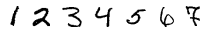
\includegraphics[align=c,width=5.3cm]{images/dataset_mnist} \\
    MNIST-M   & 32$\times$32 & 50,000 & 10,000 & & 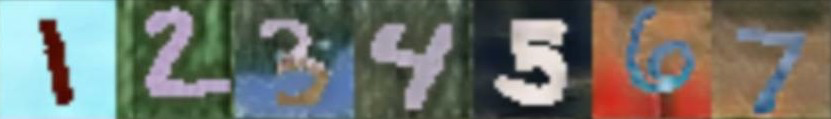
\includegraphics[align=c,width=5.3cm]{images/dataset_mnistm} \\
    SVHN   & 32$\times$32 & 73,257 & 26,032 & 531,131 & 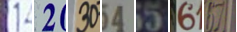
\includegraphics[align=c,width=5.3cm]{images/dataset_svhn} \\
    CIFAR-10   & 32$\times$32 & 50,000 & 10,000 & & 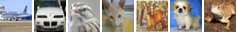
\includegraphics[align=c,width=5.3cm]{images/dataset_cifar10} \\
    STL-10   & 96$\times$96 & 1,000 & 8,000 & 100,000 & 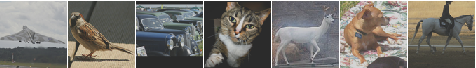
\includegraphics[align=c,width=5.3cm]{images/dataset_stl10} \\
    \bottomrule
  \end{tabular}
  \titlecaption{Overview of the datasets used}{We report the size of the images, the number of samples used for training (with only a subset of them for which we will keep the labels), the number of test samples and the number of extra images that are used only as labeled samples.}
  \label{hybridnet:tab:datasets}
\end{table}

In our experiments, we use different datasets of image classification among 10 classes. Those datasets are as follows, with additional numerical details and samples presented in \autoref{hybridnet:tab:datasets}:
\begin{itemize}
  \setlength\itemsep{0em}
  \item \textbf{MNIST} \citep{lecun}, is a simple and historical dataset that contains black and white hand-written digits.
  \item \textbf{MNIST-M} \citep{Ganin2015}, is an interesting variant of MNIST constructed artificially, initially to test domain adaptation models. In this dataset, textures and colors taken from natural images are added to MNIST digits to introduce variability. This additional information is non-discriminative and should be represented by $E_u$.
  \item \textbf{SVHN} \citep[Street View House Numbers, by][]{netzer2011reading}, contains cropped photos of house plate numbers taken by Google Street View cars. It is thus a digits dataset with a much larger variability (camera angle, colors, textures, noise, \etc) than MNIST, and is thus more difficult.
  \item \textbf{CIFAR-10} \citep{cifar10} is a dataset of natural images that cover 10 classes (airplane, automobile, bird, cat, deer, dog, frog, horse, ship, truck). It is more complicated than the previous ones due to the high variability of the natural images. It can be seen as a small ImageNet dataset since CIFAR-10 pictures are taken from ImageNet and have been resized to 32$\times$32 pixels.
  \item \textbf{STL-10} \citep{Coates2011} is the most challenging dataset. It uses the same classes as CIFAR-10 but with different images of higher resolution. Designed for \ac{SSL}, only a small number of labeled images are provided, with a large number of additional images that are unlabeled and taken from subclasses of the real classes (\eg animals and vehicles that are not in the 10 classes) which increases the difficulty.
\end{itemize}

For our semi-supervised experiments, we will keep $N_s$ labeled training samples (with $\nicefrac{N_s}{10}$ samples per class) while the rest of the data is kept unlabeled, as is commonly done. The value for $N_s$ varies over the experiments and will always be indicated.

\subsection{Preliminary results using SHADE}
\label{hybridnet:sec:exp_shade}

\begin{figure}[t]
	\centering
	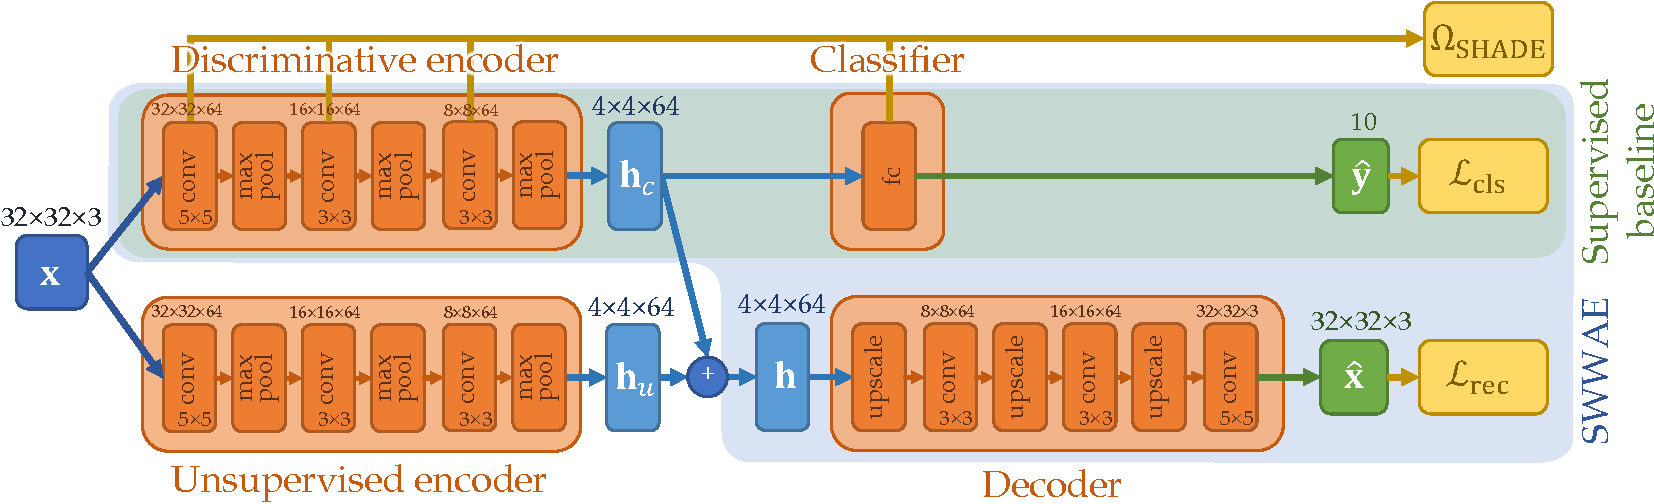
\includegraphics[width=0.95\textwidth]{images/hybridnet_withshade}
  \titlecaption{Detailed architecture of an HybridNet trained with \acs{SHADE}}{We indicate the supervised baseline (delimited in green), \acs{SWWAE} (delimited in blue) and HybridNet (whole figure) used for MNIST-M.}
    \label{hybridnet:fig:archi_shade}
\end{figure}

We first conduct preliminary experiments of HybridNet in conjunction with \ac{SHADE} in order to evaluate the effectiveness of our approach compared to existing \ac{SSL} baselines, and especially validate the idea of using a two-branch architecture. For this, we especially compare our HybridNet framework to \ac{SWWAE} by \citet{Zhao2016a}, which proposes to address the same motivations as HybridNet. \ac{SWWAE} is an \ac{AE}-based architecture for \ac{SSL} that proposes to address the problem of decoding from features made invariant because of max-pooling layers. To do so, \ac{SWWAE} uses unpooling layers in the decoder to reintroduce the pooling location and provide this missing information.

For this experiment, we start with the architecture and protocol of \citet{Zhao2016a}, illustrated in \autoref{hybridnet:fig:archi_shade} (delimited in blue). We develop an HybridNet version of the architecture used by \ac{SWWAE} by adding a second encoder and choose to use an early fusion strategy by merging the information in the latent space ($\vh = \vh_c + \vh_u$) by addition. We also do not use the unpooling strategy of \ac{SWWAE} and replace those with simple upsampling layers. This architecture is detailed in \autoref{hybridnet:fig:archi_shade} (full figure).


\begin{table}[t]
  \centering
  
  \begin{tabular}{@{}lccccc@{}}
    \toprule
    \hspace{0pt plus 1filll} Dataset    & \multicolumn{2}{c}{MNIST}       & \multicolumn{2}{c}{MNIST-M}     & SVHN     \\
            \cmidrule(l{8pt}r{8pt}){2-3} \cmidrule(l{8pt}r{8pt}){4-5}
    \hspace{0pt plus 1filll} Nb labeled samples $N_s$   & 100        & 1000       & 100        & 1000       & 1000 \\
  \midrule
  Supervised  baseline & 83.26          & 95.51          & 47.14          & 83.09          & 75.03    \\
  \acs{SWWAE}${}^*$          & 86.38          & 95.72          & 45.83          & 82.89          & 75.27    \\
  HybridNet no regul.    & 84.13          & 96.01          & 48.07          & 84.86          & 75.63    \\
  HybridNet + weight decay & 87.71          & 95.98          & 48.62          & 83.69          & 76.13    \\
  HybridNet + \acs{SHADE}        & \textbf{89.15} & \textbf{97.18} & \textbf{52.58} & \textbf{88.23} & \textbf{79.12} \\
  \bottomrule
  \multicolumn{6}{@{}p{0.75\textwidth}@{}}{\footnotesize{${}^*$ The results reported correspond to our reimplementation of this architecture based on the information provided in \cite{Zhao2016a}.}}
  \end{tabular}

  \titlecaption{Results of a first version of HybridNet with \acs{SHADE} compared to \acs{SWWAE}}{We compare supervised and semi-supervised baselines to HybridNet in different stability regularization setups. We report the accuracy (\%) measured on the test set of MNIST, MNIST-M and SVHN for different sizes of labeled dataset.}
  \label{hybridnet:table:shade}
\end{table}

We train the supervised baseline (without a decoder), \ac{SWWAE} and three variants of HybridNet with no stability regularization, with weight decay and with \ac{SHADE} for stability. We apply them on MNIST, MNIST-M and SVHN (see \autoref{hybridnet:tab:datasets} for image samples) and report the results in \autoref{hybridnet:table:shade}. Among the three, we can note that MNIST-M is particularly interesting to demonstrate the capabilities of HybridNet. As we can see in the image samples, it contains a lot of variability in the visual information (colors, textures) and very little semantic information useful for classification (the overall shape of the digit). HybridNet, thanks to its two latent spaces, should allow efficient separation of the two types of information.

 First, \ac{SWWAE}, our \ac{SSL} baseline, improves over the supervised-only baseline except on MNIST-M which could be explained by the fact that the reconstruction loss might produce too many features that need to encode the wide variety of textures in the dataset and does not learn features useful for classification. HybridNet without regularization usually does improve slightly over \ac{SWWAE}, which is normal since stability regularization is a key element to make this model work. Indeed, adding weight decay --\,which can be seen as adding invariance \textit{cf.} \autoref{shade:sec:noncond_entropy} \textit{``Non-conditional Entropy''}\,--, provides an interesting gain to HybridNet, increasing the accuracy on MNIST ($N_s = 100$) from 84.1\% to 87.7\%. On MNIST-M however, the gain is negligible, probably due to the non-class-conditional nature of weight decay. Indeed, using \ac{SHADE} for stability provides an important gain, especially on MNIST-M where we gain $\sim$4\,pts over the HybridNet baseline $\sim$6\,pts over the supervised and \ac{SSL} baselines.

 \begin{figure}[t]
  \centering
  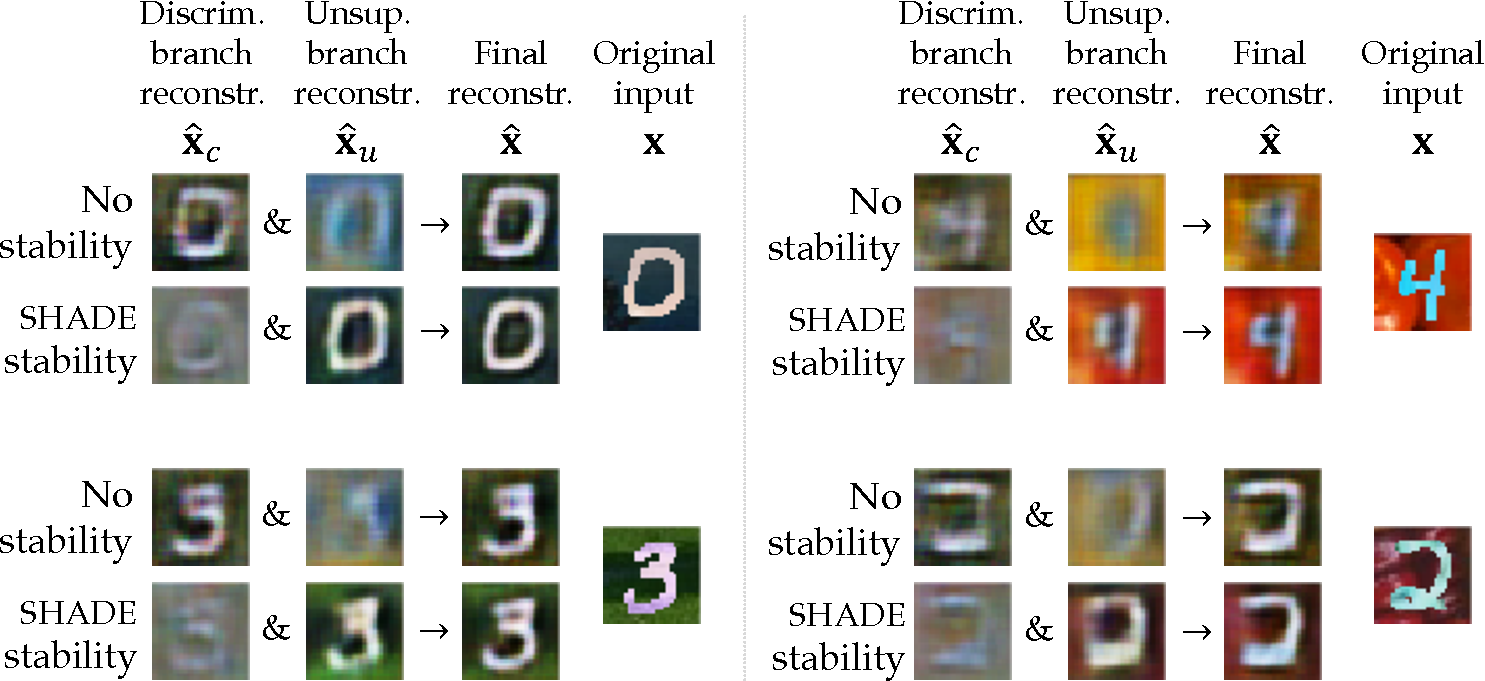
\includegraphics[width=1\textwidth]{images/hybridnet_withshade_samples}
  \titlecaption{Reconstructions of samples from MNIST-M by HybridNet with and without \acs{SHADE}}{We show the final reconstruction $\vxh = D(\vh) = D(\vh_c + \vh_u)$ and the ``partial'' reconstructions $\vxh_c = D(\vh_c)$ and $\vxh_u = D(\vh_u)$ produced when feeding the decoder with the features from a single branch.}
    \label{hybridnet:fig:samples_with_shade}
\end{figure}

With \autoref{hybridnet:fig:samples_with_shade}, we propose to visualize the effect of using \ac{SHADE} in HybridNet on MNIST-M. We show, for four different images, the final reconstruction $\vxh = D(\vh) = D(\vh_c + \vh_u)$ and partial reconstructions $\vxh_c = D(\vh_c)$ and $\vxh_u = D(\vh_u)$. This is shown for two HybridNet models, trained with and without \ac{SHADE} as a stability regularizer.
One can see that the full reconstructions $\vxh$ with \textit{\ac{SHADE}} are quite better than the ones with \textit{no stability} regularization, particularly in terms of color integrity and texture quality. This can be analyzed by looking at the contribution of each branch through $\vxh_c$ and $\vxh_u$. For the HybridNet with \ac{SHADE}, we observe that the details (color, texture, \etc) are encoded in the unsupervised branch $\vh_u$ as desired, while the discriminative branch $\vh_c$ barely contains the shape of the digit. This is not the case without regularization where the information does not seem to be organized, which is particularly visible on the bottom digits \textit{2} and \textit{3} where the green and red backgrounds are almost lost without stability.

In this experiment, we validated the relevance of using a two-branch architecture to improve on existing techniques based on \ac{AE}, in particular \ac{SWWAE}. We also show how adding a regularization encouraging invariance, namely \ac{SHADE}, can work in concert with the two-branch architecture to effectively separate the information.

\paragraph{Discussion.} While it made sense to reuse our work on invariance with \ac{SHADE} in HybridNet, we now propose to discuss its viability as a regularizer in this context. During this first experiment, we observed that, while effective, \ac{SHADE} was too strong of a regularizer toward invariant representations, making it difficult for representations from $E_c$ to cooperate with reconstruction. Furthermore, \ac{SHADE} is designed with the idea that the model trained with a supervision signal is able to produce relevant class-related representations that we model with a binary latent code $\vz$, \cf \autoref{shade:sec:dev}, $\vz$ being a sort of surrogate of $\vy$ for class information, to compute a replacement of $\Ent(\vh_c \mid \vy)$. In the context of \ac{SSL} where we only have very few labels to learn those latent codes $\vz$, it is not certain how \ac{SHADE} will behave. For this reason and in order to more easily compare HybridNet with state-of-the-art methods, we choose to replace \ac{SHADE} with stability methods like Mean Teacher \citep{Tarvainen2017}.

In addition, these experiments confirmed that controlling the behavior of an early fusion HybridNet was complicated and very sensitive to hyperparameters values. This is why the rest of the experiments will use a late fusion strategy, replacing the single decoder by two decoders, one for each branch, to provide more control over the behavior of the model as explained in \autoref{hybridnet:sec:training}, \textit{``Branch cooperation''}.

\begin{figure}[t]
	\centering
	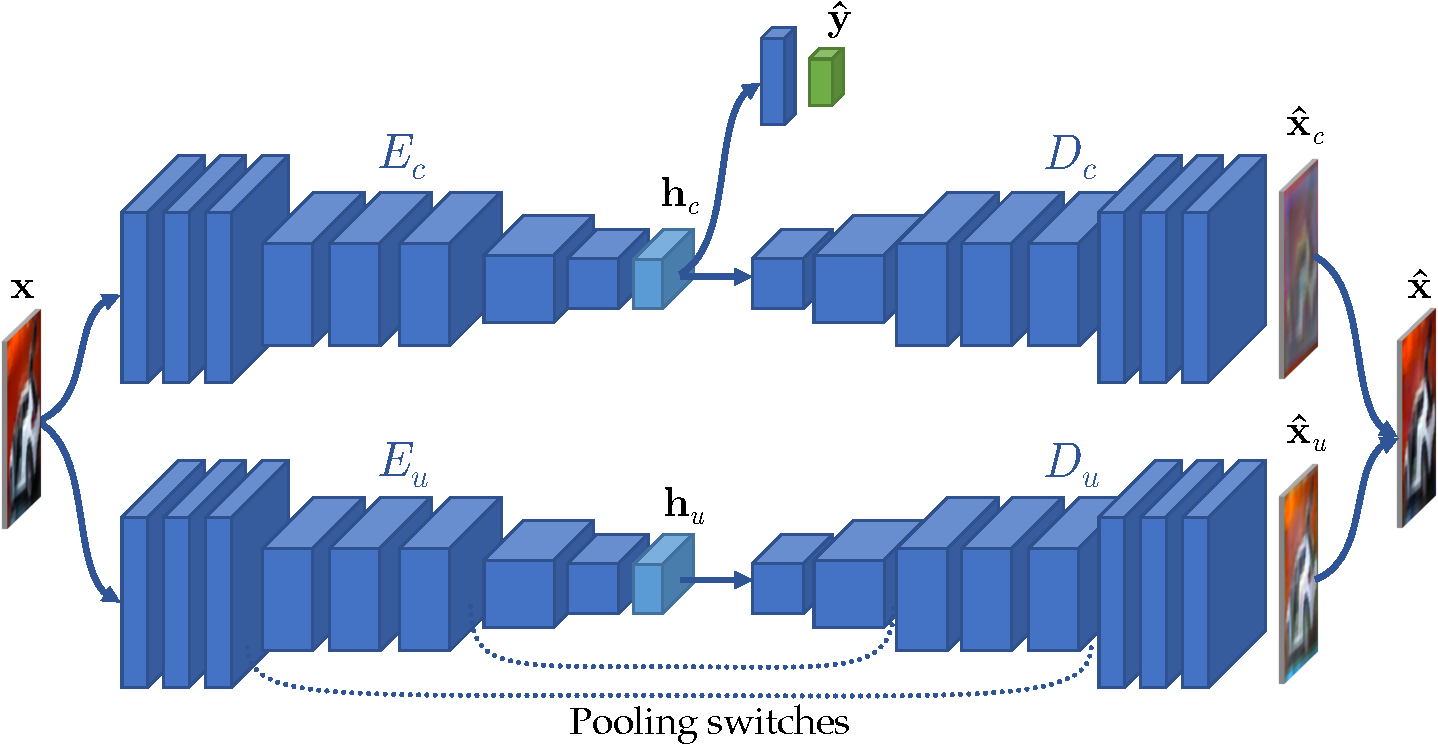
\includegraphics[width=0.9\textwidth]{images/hybridnet_convlarge}
  \titlecaption{Example of a HybridNet architecture}{The original classifier (ConvLarge) constitutes $E_c$ and has been mirrored to create $D_c$ and duplicated for $E_u$ and $D_u$, with the addition of unpooling in the discriminative branch.}
    \label{hybridnet:fig:cifar10-archi}
\end{figure}

\begin{table}[p]
  \centering
  \begin{tabular}{ l l l}
  \toprule
  \multicolumn{3}{c}{\textbf{Encoders $E_c$ and $E_u$}} \\
  \midrule
  Input & $\tilde\vx$ & $32\times 32\times 3$ \\
  Convolution & $128$ filters, $3\times3$, padding $1$ & $32\times 32\times 128$ \\
  Convolution & $128$ filters, $3\times3$, padding $1$ & $32\times 32\times 128$ \\
  Convolution & $128$ filters, $3\times3$, padding $1$ & $32\times 32\times 128$ \\
  Pooling   & Maxpool $2\times2$ & $16\times 16\times 128$ \\
  Dropout   & $p=0.5$  & $16\times 16\times 128$ \\
  Convolution & $256$ filters, $3\times3$, padding $1$  & $16\times 16\times 256$ \\
  Convolution & $256$ filters, $3\times3$, padding $1$  & $16\times 16\times 256$ \\
  Convolution & $256$ filters, $3\times3$, padding $1$  & $16\times 16\times 256$ \\
  Pooling & Maxpool $2\times2$  & $8\times 8\times 256$ \\
  Dropout & $p=0.5$  & $8\times 8\times 256$ \\
  Convolution & $512$ filters, $3\times3$, padding $0$  & $6\times 6\times 512$ \\
  Convolution & $256$ filters, $1\times1$, padding $1$ & $6\times 6\times 256$ \\
  Convolution & $128$ filters, $1\times1$, padding $1$ & $6\times 6\times 128$ \\
  Output & $\vh_c$ or $\vh_u$ & $6\times 6\times 128$ \\
  
  \toprule
  \multicolumn{3}{c}{\textbf{Classifier $C$}}\\
  \midrule
  Input & $\vh_c$& $6\times 6\times 128$ \\
  Pooling & Global average pool & $1\times 1\times 128$ \\
  Fully connected & with Softmax & $10$ \\
  Output & $\vyh$ & $10$ \\
  \toprule
  \multicolumn{3}{c}{\textbf{Decoders $D_c$ and $D_u$}}\\
  \midrule
  Input & $\vh_c$ or $\vh_u$ & $6\times 6\times 128$ \\
  TConvolution & $256$ filters, $1\times1$, padding $1$  & $6\times 6\times 256$ \\
  TConvolution & $512$ filters, $1\times1$, padding $1$  & $6\times 6\times 512$ \\
  TConvolution & $256$ filters, $3\times3$, padding $0$  & $8\times 8\times 256$ \\
  Upsampling   & $2\times2$ (unpooling in $D_u$)  & $16\times 16\times 256$ \\
  TConvolution & $256$ filters, $3\times3$, padding $1$ & $16\times 16\times 256$ \\
  TConvolution & $256$ filters, $3\times3$, padding $1$ & $16\times 16\times 256$ \\
  TConvolution & $128$ filters, $3\times3$, padding $1$ & $16\times 16\times 128$ \\
  Upsampling & $2\times2$ (unpooling in $D_u$) & $32\times 32\times 128$ \\
  TConvolution & $128$ filters, $3\times3$, padding $1$  & $32\times 32\times 128$ \\
  TConvolution & $128$ filters, $3\times3$, padding $1$  & $32\times 32\times 128$ \\
  TConvolution & $3$ filters, $3\times3$, padding $1$  & $32\times 32\times 3$ \\
  Output & $\vxh_c$ or $\vxh_u$ & $32\times 32 \times 3$ \\
  \bottomrule
  \end{tabular}
  \titlecaption{Architecture of HybridNet version of ConvLarge for CIFAR-10}{This architecture is also presented visually in \autoref{hybridnet:fig:cifar10-archi}. The original ConvLarge model corresponds to $C\circ E_c$. TConvolution stands for ``transposed convolution'' \citep{dumoulin2016guide}. Each Convolution or TConvolution is followed by a Batch Normalization layer and a LeakyRELU of parameter $\alpha = 0.1$.}
  \label{hybridnet:table:convlarge}
  \end{table}

\subsection{HybridNet framework validation}
\label{hybridnet:sec:as}

We now propose a thorough analysis of the behavior of our model at two different levels: first by comparing it to baselines that we obtain when disabling parts of the architecture, and second by analyzing the contribution of the different terms of the training loss of HybridNet both quantitatively and through visualizations.

This study is performed based on the ConvLarge architecture introduced by \citet{Rasmus2015} on CIFAR-10. This is the most common setup used in recent \ac{SSL} experiments \citep{Sajjadi2016,Laine2016,Tarvainen2017}. This is a fairly simple \ac{ConvNet} architecture, resembling VGG \citep{simonyan2015very}, with blocks of convolutions followed by max-poolings.

We detail this architecture in \autoref{hybridnet:table:convlarge} and represent it schematically in \autoref{hybridnet:fig:cifar10-archi}, in its HybridNet version. The design of the HybridNet version of ConvLarge follows \autoref{hybridnet:sec:model} and uses Temporal Ensembling \citep{Laine2016} to produce stability targets $\tilde{\vy}$. We also use an adapted version of ConvLarge for STL-10 with added blocks of convolutions and pooling to obtain additional visualizations and quantitative results.

Models are trained with Adam with a learning rate of 0.003 for 600 epochs with batches of 20 labeled images and 80 unlabeled ones. The various loss-weighting terms $\lambda$ of the general loss (\autoref{hybridnet:eq:full-loss}) were set so that the different loss terms have values of the same order of magnitude. Thus, all $\lambda$ were set to either 0 or 1 if activated or not, except $\lambda_s$ set to 0 or 100. The details of the architecture and hyperparameters values are provided in \autoref{chapter:hybridnetA}.


\subsubsection{Ablation study of the architecture}

We start this analysis by validating our architecture with an ablation study on CIFAR-10 with different number of labeled samples. By disabling parts of the model and training terms, we compare HybridNet to different baselines and validate the importance of combining both contributions of the paper: the architecture and the training method.

Results are presented in \autoref{hybridnet:table:ablation}. The classification and auto-encoder results are obtained with the same code and hyperparameters by simply disabling different losses and parts of the model: the classifier only uses $E_c$ and $C$; and the auto-encoder \citep[similar to][]{Zhao2016a} only $E_c$, $D_c$ and $C$. For both, we can add the stability loss. The HybridNet architecture only uses the classification and reconstructions loss terms while the second result uses the full training loss.


\begin{table}[t]
  \centering
  \begin{tabular}{llll}
    \toprule
                                              & \multicolumn{3}{c}{Labeled samples $N_s$}           \\ \cmidrule{2-4}
Model                                         & 1000          & 2000          & 4000          \\ \midrule
Classification                                & 63.4          & 71.5          & 79.0          \\
Classification and stability                  & 65.6          & 74.6          & 81.3          \\ \cmidrule{1-4}
Auto-encoder                                & 65.0          & 73.6          & 79.8          \\
Auto-encoder and stability                  & 71.8          & 80.4          & 84.9          \\ \cmidrule{1-4}

HybridNet architecture                        & 63.2          & 74.0          & 80.3          \\
HybridNet architecture and full training loss & \textbf{74.1} & \textbf{81.6} & \textbf{86.6} \\ \bottomrule
  \end{tabular}

  \titlecaption[c]{Ablation study}{performed on CIFAR-10 with ConvLarge architecture.}
  \label{hybridnet:table:ablation}
\end{table}


First, we can see that the HybridNet architecture alone already yields an improvement over the baseline and the auto-encoder, except at 1000 labels. This could be explained by the fact that with very few labels, the model fails to correctly separate the information between the two branches because of the faint classification signal, and the additional loss terms that control the training of HybridNet are even more necessary. Overall, the architecture alone does not provide an important gain since it is not guided to efficiently take advantage of the two branches, indeed, we see that the addition of the complete HybridNet loss allows the model to provide much stronger results, with an improvement of 6-7\,pts over the architecture alone, around 5-6\,pts better than the stability or auto-encoding baseline, and 7-10\,pts more than the supervised baseline. The most challenging baseline is the stabilized auto-encoder that manages to take advantage of the stability loss but from which we still improve by 1.2-2.8\,pts.

This ablation study demonstrates the capability of the HybridNet framework to surpass the different architectural baselines, and shows the importance of the complementarity between the two-branch architecture and the complete training loss.




\colorlet{verylightgray}{gray!20}
\newcommand{\rowmidlinewc}{\arrayrulecolor{verylightgray}\cmidrule{1-8}
            \arrayrulecolor{black}}
\newcommand{\rowmidlinewcb}{\arrayrulecolor{verylightgray}\cmidrule{1-5}
            \arrayrulecolor{black}}

\newcommand{\spa}{\quad\,}
\newcommand{\spb}{\qquad\,}

\begin{table}[p]
  \begin{subtable}[t]{\linewidth}
    \centering
    \begin{tabular}{@{}lclllll@{\hspace{1cm}}cc}
    \toprule
    & &\rotb{$\mathcal L_\mathrm{classif}$} & \rotb{$\Omega_\mathrm{stability}$} & \rotb{$\mathcal L_\mathrm{rec}$ {\scriptsize(hybrid)}} & \rotb{$\mathcal L_\mathrm{rec-inter}$} & \rotb{$\mathcal L_\mathrm{rec-balanced}$} & CIFAR-10 & STL-10 \\
    \midrule
    \multirow{2}{*}{\ \ \ cls.}
    & \scriptsize \textit{a} & \OK &     &     &     &    & 71.5 & 65.6         \\
    & \scriptsize \textit{b} &\OK & \OK &     &     &    & 74.6 & 69.8         \\
    \rowmidlinewc
    \multirow{3}{*}{\begin{tabular}{@{}l@{}}\ \ \  cls. \\ + rec.\end{tabular}}
    & \scriptsize \textit{c} &\OK &     & \OK &     &    & 72.4 & 67.8         \\
    & \scriptsize \textit{d} &\OK &     & \OK & \OK &    & 74.0 & --         \\
    & \scriptsize \textit{e} &\OK &     & \OK & \OK & \OK & 75.2 & --         \\
    \rowmidlinewc
  \multirow{4}{*}{\begin{tabular}{@{}l@{}}\ \ \ cls. \\ + rec.\\ + stab.\end{tabular}}
    & \scriptsize \textit{f} &\OK & \OK & \OK &     &    & 77.7 & 71.5           \\
    & \scriptsize \textit{g} &\OK & \OK & \OK &     & \OK & 77.4 & --         \\
    & \scriptsize \textit{h} &\OK & \OK & \OK & \OK &    & 80.8 & 72.2          \\
    & \scriptsize \textit{i} &\OK & \OK & \OK & \OK & \OK & \textbf{81.6} & \textbf{74.1} \\
     \bottomrule
  \end{tabular}

  \caption{\textbf{Quantitative results} obtained with ConvLarge on CIFAR-10 with 2000 labeled samples and ConvLarge-like on STL-10 with 1000 labeled samples.}
  \label{hybridnet:table:as-scores}
  \end{subtable}

  \vspace*{1.3em}
  \begin{subtable}[t]{\linewidth}
	\centering
  \renewcommand{\arraystretch}{1.74}
    \begin{tabular}{@{}cllllc@{}}
    \toprule
    &\rotb{$\mathcal L_\mathrm{rec}$ {\scriptsize(hybrid)}} & \rotb{$\mathcal L_\mathrm{rec-inter}$} & \rotb{$\mathcal L_\mathrm{rec-balanced}$} & \rotb{$\Omega_\mathrm{stability}$} &
    $\vx \spa \vxh_c \spa \vxh_u \spa \vxh \spb \vx \spa \vxh_c \spa \vxh_u \spa \vxh \spb \vx \spa \vxh_c \spa \vxh_u \spa \vxh $ \\ \midrule
    \scriptsize \textit{c} &\OK &     &     &     & \multirow{8}{*}{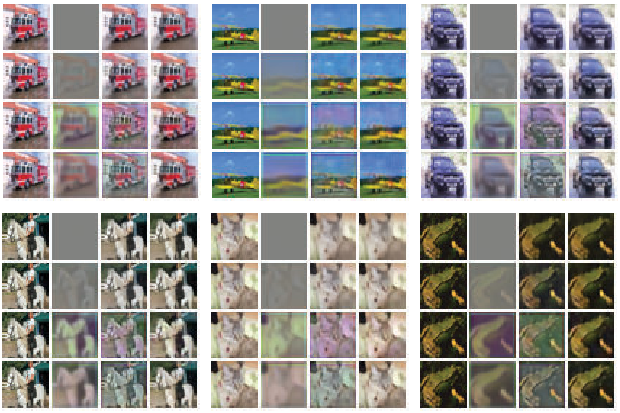
\includegraphics[width=11cm]{images/hybridnet_viz-as-simple.pdf}\!}          \\
    \scriptsize \textit{d} &\OK & \OK    &     &     &           \\
    \scriptsize \textit{e} &\OK & \OK    & \OK    &     &           \\
    \scriptsize \textit{i} &\OK & \OK    & \OK    & \OK    &           \\
    \rowmidlinewcb
    \scriptsize \textit{c} & \OK &        &     &     &           \\
    \scriptsize \textit{d} &\OK & \OK    &     &     &           \\
    \scriptsize \textit{e} &\OK & \OK    & \OK    &     &           \\
    \scriptsize \textit{i} &\OK & \OK    & \OK    & \OK    &           \\
     \bottomrule
  \end{tabular}
  \caption{\textbf{Visual results on CIFAR-10 for four model variants.} We show the input $\vx$, full ($\vxh$) and partial ($\vxh_c$ and $\vxh_u$) reconstructions. With only reconstruction, the visual information by-passes the discriminative branch and is completely captured by $\vxh_u$. The different terms improve the organization of the information between both branches.
  }
  \label{hybridnet:table:asviz}
\end{subtable}

  \titlecaption[c]{Detailed ablation studies}{when activating different terms and techniques of the HybridNet learning.}
  \label{hybridnet:table:abl}
\end{table}



\subsubsection{Importance of the various loss terms}

We now propose a more fine-grain study to look at the importance of each loss term of the HybridNet training described in \autoref{hybridnet:sec:training}, both through classification results and visualizations.

First, in \autoref{hybridnet:table:as-scores} we show the classification accuracy on CIFAR-10 with 2000 labels and STL-10 with 1000 labels for numerous combinations of loss terms. These results demonstrate that each loss term has its importance and that all of them cooperate in order to reach the final best result of the full HybridNet model. In particular, the stability loss is an important element of the training but is not sufficient as shown by lines \textit{b} and \textit{f-h}, while the other terms bring an equivalent gain as shown by lines \textit{c-e}. Both those $\sim$5\,pts gains can be combined to work in concert and reach the final score line \textit{i} of a $\sim$10\,pts gain.

Second, to interpret how the branches behave we propose to visualize the different reconstructions $\vxh_c$, $\vxh_u$ and $\vxh$ for different combinations of loss terms in \autoref{hybridnet:table:asviz}. With only the final reconstruction term (lines \textit{c}), the discriminative branch does not contribute to the reconstruction and is thus barely regularized by the reconstruction loss, showing little gain over the classification baseline. The addition of the intermediate reconstruction terms helps the discriminative branch to produce a weak reconstruction (lines \textit{d}) and is complemented by the branch balancing technique (lines \textit{e}) to produce balanced reconstructions in both branches. The stability loss (lines \textit{i}) adds little visual impact on $\vxh_c$, it has probably more impact on the quality of the latent representation $\vh_c$ and seems to help in making the discriminative features and classifier more robust with a large improvement of the accuracy.


\begin{figure}[t]
	\centering
	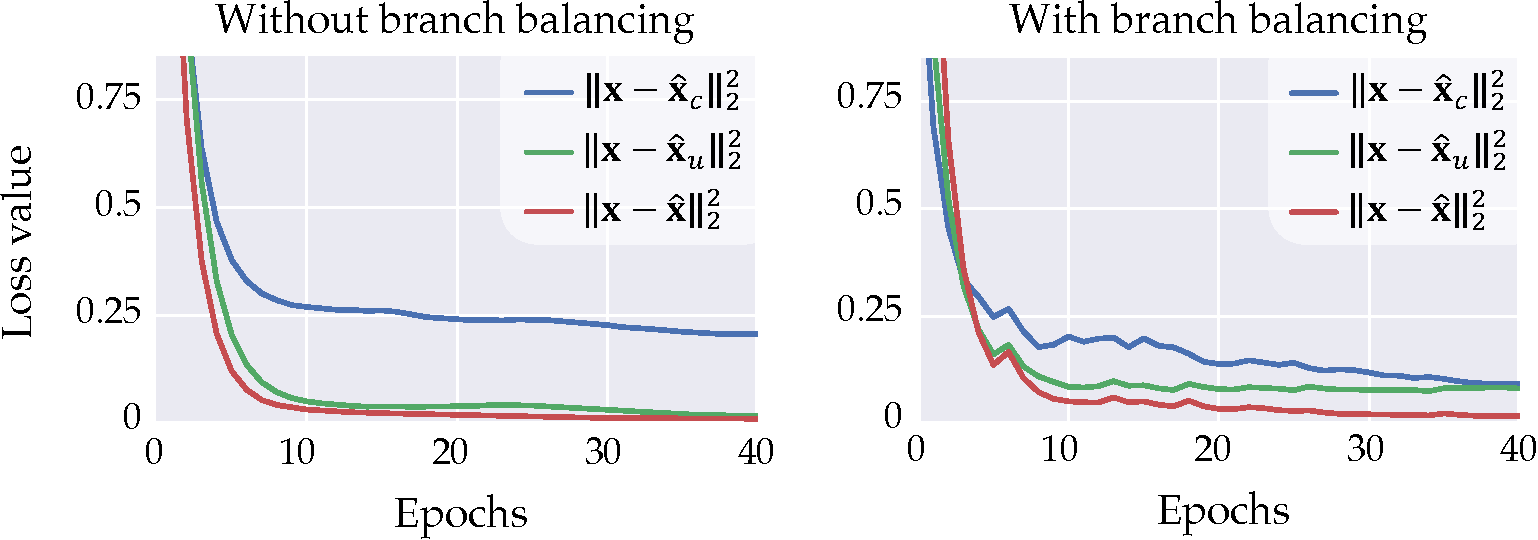
\includegraphics[width=0.93\textwidth]{images/hybridnet_recloss}
  \titlecaption{Evolution of reconstruction losses with and without branch balancing}{Without branch balancing, $\vxh_u$ reconstructs $\vx$ alone and $E_c$ receives little regularization signal. Using branch balancing makes both branches contribute to the reconstruction in comparable magnitude.}
    \label{hybridnet:fig:recloss}
\end{figure}

Another way to see the effect of the branch balancing term is by looking at the evolution of the partial reconstruction losses ($||\vx - \vxh_c||_2^2$ and $||\vx - \vxh_u||_2^2$) that measure how much each branch is contributing to the final reconstruction $||\vx - \vxh||_2^2$. We do so during the training of a HybridNet with and without branch balancing and show the result in \autoref{hybridnet:fig:recloss}: without it, we can see that $||\vxh_u - \vx||_2^2 \approx 0$ so the unsupervised branch is reconstructing almost alone; with it, the two branches do not reconstruct perfectly which enables their cooperation, as expected.


\begin{figure}[t]
	\centering
	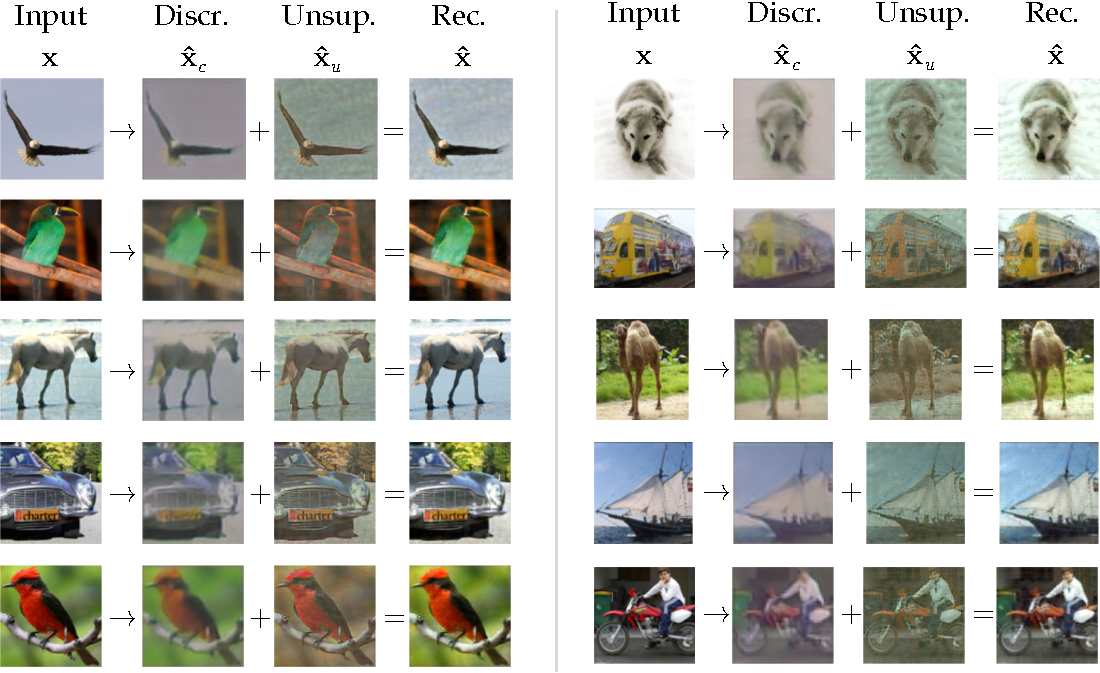
\includegraphics[width=\textwidth]{images/hybridnet_viz-stl}
  \titlecaption[c]{Visualizations of input, partial and final reconstructions}{of STL-10 images using a HybridNet model derived from a ConvLarge-like architecture.}
    \label{hybridnet:fig:viz-stl}
\end{figure}

\subsubsection{Visualization of information separation on CIFAR-10 and STL-10}


Overall, we can see in \autoref{hybridnet:table:asviz} lines \textit{i} that thanks to the full HybridNet training loss, the information is correctly separated between $\vxh_c$ and $\vxh_u$ than both contribute somewhat equally while specializing on different types of information. For example, for the blue car, $\vxh_c$ produces a blurry car with approximate colors, while $\vxh_u$ provides both shape details and exact color information. For nicer visualizations, we also show reconstructions of the full HybridNet model trained on STL-10, which has larger images, in \autoref{hybridnet:fig:viz-stl}. These confirm the observations on CIFAR-10. HybridNet is able to produce a very good final reconstruction composed of a rough reconstruction that lacks texture and color details from the discriminative branch, completed by low-level details of shape, texture, writings, color correction and background information from the unsupervised branch.



\renewcommand{\leftmark}{\spacedlowsmallcaps{Separating Discriminative and Non-Discriminative Information}}
\begin{sidewaystable}[p]
  \centering
  \begin{tabular}{@{}llrrrrrr@{}}
    \toprule
    & \hspace{0pt plus 1filll} Dataset                                    & \multicolumn{3}{c}{CIFAR-10} & \multicolumn{2}{c}{SVHN} & STL-10 \\
    \cmidrule(l{4pt}r{4pt}){3-5} \cmidrule(l{4pt}r{4pt}){6-7} \cmidrule(l{4pt}r{4pt}){8-8}
    Model type & Model \hspace{0pt plus 1filll} Nb. labeled images $N_s$ & 1000  & 2000 & 4000 & 500 & 1000 & \multicolumn{1}{c}{1000} \\
    \midrule
  \multirow{4}{*}{\begin{tabular}{@{}c@{}}Reconstruction /\\ Generation \\ based\end{tabular}}
    & SWWAE \footnotesize\citep{Zhao2016a}                         &   &   &   & & 23.56 & 25.67 \\
    & Ladder Network \footnotesize\citep{Rasmus2015}                  &&       & 20.40      \\
    & Improved GAN \footnotesize\citep{Salimans2016}              & 21.83 & 19.61 & 18.63 & 18.44 & 8.11 &  \\
    & CatGAN \footnotesize\citep{Springenberg2015}                    &&       & 19.58      \\

    \cmidrule{1-8}
    \multirow{4}{*}{Stability based}
    & Stability regularization \footnotesize\citep{Sajjadi2016}    &&       & 11.29  & 6.03 & &      \\
    & Temporal Ensembling \footnotesize\citep{Laine2016}           &&       & 12.16 & 5.12 & 4.42  \\
    & Mean Teacher ConvLarge \footnotesize\citep{Tarvainen2017}              & 21.55 & 15.73 & 12.31 & 4.18 & 3.95 \\
    & Mean Teacher ResNet \footnotesize\citep{Tarvainen2017}          & 10.10  &      & 6.28 & ${}^*$2.33 & ${}^*$2.05 & ${}^*$16.8        \\
    
    \cmidrule{1-8}

    & ResNet baseline \footnotesize\citep{Gastaldi2017}						 & 45.2 & 24.3 & 15.45 & 12.27 & 9.56 & 18.0  \\
    Rec. \& Stability & \textbf{HybridNet [ours]}  & \textbf{8.81} & \textbf{7.87} & \textbf{6.09} & \textbf{1.85} & \textbf{1.80} & \textbf{15.9} \\
    
    \bottomrule
  \end{tabular}

  \titlecaption{Results using a ResNet-based HybridNet}{trained on CIFAR-10, STL-10 and SVHN. ``Mean Teacher ResNet'' is our classification \& stability baseline; results marked with ${}^*$ are not reported in the original paper and were obtained ourselves. %by simply disabling HybridNet components of the model
  }
  \label{hybridnet:table:cifar10}
\end{sidewaystable}


\subsection{State-of-the-art comparison}
\label{hybridnet:sec:cifar10sota}

After studying the behavior of this novel architecture, we propose to demonstrate its effectiveness and capability to produce state-of-the-art results for \ac{SSL} on three datasets: SVHN, CIFAR-10 and STL-10.

We use ResNet architectures to constitute the supervised encoder $E_c$ and classifier $C$; and augment them with a mirror decoder $D_c$ and an unsupervised second branch containing an encoder $E_u$ and a decoder $D_u$ using the same architecture. For SVHN and CIFAR-10, we use the small ResNet from \citep{Gastaldi2017}, which is used in Mean Teacher \citep{Tarvainen2017} and currently achieves state-of-the-art results on CIFAR-10. For STL-10, we upscale the images to 224$\times$224\,px and use a regular ResNet-50 pretrained on the Places dataset.

We trained HybridNet with the training method described in \autoref{hybridnet:sec:training}, using Mean Teacher to produce stability targets $\tilde{\vy}\kk$. The training protocol follows exactly the protocol of Mean Teacher \citep{Tarvainen2017} for CIFAR-10 and a similar one for SVHN and STL-10 for which \citep{Tarvainen2017} does not report results with ResNet. The hyperparameters added in HybridNet, \textit{i.e.} the weights of the reconstruction terms (final and intermediate), were coarsely adjusted on a validation set. The details of the architecture used and the values of the hyperparameters are provided in \autoref{chapter:hybridnetA}.

The results of these experiments are presented in \autoref{hybridnet:table:cifar10}.
We can see the huge performance boost obtained by HybridNet compared to the ResNet baselines, in particular with CIFAR-10 with 1000 labels where the error rate goes from 45.2\% to 8.81\%, which demonstrates the large benefit of our regularizer. HybridNet also improves over the strong Mean Teacher baseline \citep{Tarvainen2017}, with an improvement of 1.29\,pt with 1000 labeled samples on CIFAR-10, and 0.9\,pt on STL-10. We also significantly improve over other stability-based approaches \citep{Sajjadi2016,Laine2016}, and over the Ladder Networks \citep{Rasmus2015} and GAN-based techniques \citep{Springenberg2015,Salimans2016}.

These results demonstrate the capability of HybridNet to apply to large residual architectures --\,that are very common nowadays\,-- and to improve over baselines that already provided very good performance.


\section{Conclusion}

In this chapter, we proposed to go further in the development of new ways to represent the information in a \acf{ConvNet}, tackling the issue of \acf{SSL}. In this context, one can usually use regularization techniques like \ac{SHADE} or stability techniques which propose to increase the invariance of the representation, but this comes in conflict with a reconstruction task that is often used to leverage unlabeled data in \ac{SSL}.

To overcome this incompatibility and encourage efficient cooperation between the two tasks, we proposed HybridNet, an auto-encoder-based architecture with two distinct paths that separate the discriminative information useful for classification from the remaining information that is only useful for reconstruction. By adding this new unsupervised branch, we are able to release the constraints imposed by reconstruction and structure the information between the two latent spaces. This is achieved by the loss terms and training technique that accompany the architecture and allow it to behave in the desired way. In the experiments, we validated the significant performance boost brought by HybridNet in comparison with several other common architectures that use reconstruction losses and stability. We also showed that HybridNet can produce state-of-the-art results on CIFAR-10, STL-10 and SVHN.

While HybridNet was developed for the particular case of \ac{SSL}, this idea of a two-branch architecture that makes classification and reconstruction cooperate can also be interesting in a wider variety of contexts. In the next chapter, we consider the problem of using a two-branch architecture to encode two complementary \textit{semantic} information --\,thus using early fusion for a more complex combination\,-- from which we can reconstruct an image.
